\paragraph{QuizziPedia::Back-End::App::Controllers::TopicController}
\label{QuizziPedia::Back-End::App::Controllers::TopicController}
\begin{figure}[ht]
	\centering
	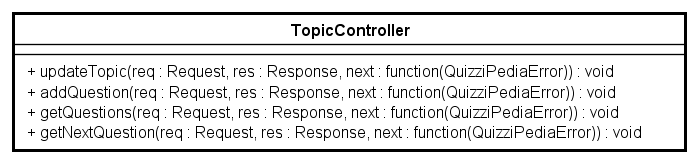
\includegraphics[scale=0.8]{UML/Classi/Back-End/QuizziPedia_Back-End_App_Controllers_topicController.png}
	\caption{QuizziPedia::Back-End::App::Controllers::TopicController}
\end{figure}
\FloatBarrier
\begin{itemize}
	\item \textbf{Descrizione}:
	classe che gestisce la logica applicativa riguardante la visualizzazione e la modifica degli argomenti delle domande;
	\item \textbf{Utilizzo}:
	viene utilizzata per implementare le funzionalità necessarie a gestire le richieste \textit{REST\ped{G}} legate agli argomenti delle domande;
	\item \textbf{Relazioni con altre classi}:
		\begin{itemize}
			\item \textbf{IN \texttt{QuestionRouter}}:
			classe che gestisce le richieste relative alle operazioni riguardanti le domande. Componente \textit{ConcreteHandler\ped{G}} del \textit{design pattern\ped{G}} \textit{Chain of responsibility\ped{G}};
			\item \textbf{OUT \texttt{TopicModel}}: 
			classe che modella gli argomenti delle domande.
		\end{itemize}
	\item \textbf{Metodi}:
		\begin{itemize}
			\item \texttt{+ updateStatisticTopic(req : Request, res : Response, \\next : function(QuizziPediaError)): void} \\
			Aggiorna il numero di risposte esatte e totali date a domande sull'argomento da parte degli utenti. \\
			\textbf{Parametri}:
			\begin{itemize}
			\item \texttt{req: Request} \\
			Rappresenta la richiesta inviata al \textit{server\ped{G}}. Contiene l'identificativo dell'argomento da aggiornare e l'informazione di se è stata data o meno una risposta corretta alla domanda su quell'argomento;
			\item \texttt{res: Response} \\
			Rappresenta la risposta che il \textit{server\ped{G}} fornirà al termine dell'esecuzione del metodo;
			\item \texttt{next: function(QuizziPediaError)} \\
			Rappresenta la \textit{callback\ped{G}} che il metodo deve chiamare al termine dell'elaborazione per passare il controllo ai successivi \textit{middleware\ped{G}}. La presenza del parametro facoltativo QuizziPediaError attiva la catena di gestione dell'errore in sostituzione della normale catena di gestione delle richieste.
			\end{itemize}
			\item \texttt{+ getNextQuestion(req : Request, \\res : Response, next : function(QuizziPediaError)): void} \\
			Restituisce la domanda successiva di un allenamento.  \\
			\textbf{Parametri}:
			\begin{itemize}
			\item \texttt{req: Request} \\
			Rappresenta la richiesta inviata al \textit{server\ped{G}}. Contiene l'identificativo dell'argomento trattato nell'allenamento e il livello dell'utente che lo sta svolgendo;
			\item \texttt{res: Response} \\
			Rappresenta la risposta che il \textit{server\ped{G}} fornirà al termine dell'esecuzione del metodo;
			\item \texttt{next: function(QuizziPediaError)} \\
			Rappresenta la \textit{callback\ped{G}} che il metodo deve chiamare al termine dell'elaborazione per passare il controllo ai successivi \textit{middleware\ped{G}}. La presenza del parametro facoltativo QuizziPediaError attiva la catena di gestione dell'errore in sostituzione della normale catena di gestione delle richieste.
			\end{itemize}
			\item \texttt{+ getTopics(req : Request, \\res : Response, next : function(QuizziPediaError)): void} \\
			Restituisce gli argomenti presenti nel sistema.  \\
			\textbf{Parametri}:
			\begin{itemize}
			\item \texttt{req: Request} \\
			Rappresenta la richiesta inviata al \textit{server\ped{G}};
			\item \texttt{res: Response} \\
			Rappresenta la risposta che il \textit{server\ped{G}} fornirà al termine dell'esecuzione del metodo;
			\item \texttt{next: function(QuizziPediaError)} \\
			Rappresenta la \textit{callback\ped{G}} che il metodo deve chiamare al termine dell'elaborazione per passare il controllo ai successivi \textit{middleware\ped{G}}. La presenza del parametro facoltativo QuizziPediaError attiva la catena di gestione dell'errore in sostituzione della normale catena di gestione delle richieste.
			\end{itemize}
			\item \texttt{+ getKeywords(req : Request, \\res : Response, next : function(QuizziPediaError)): void} \\
			Restituisce tutte le keywords delle domande di un singolo argomento.  \\
			\textbf{Parametri}:
			\begin{itemize}
			\item \texttt{req: Request} \\
			Rappresenta la richiesta inviata al \textit{server\ped{G}};
			\item \texttt{res: Response} \\
			Rappresenta la risposta che il \textit{server\ped{G}} fornirà al termine dell'esecuzione del metodo;
			\item \texttt{next: function(QuizziPediaError)} \\
			Rappresenta la \textit{callback\ped{G}} che il metodo deve chiamare al termine dell'elaborazione per passare il controllo ai successivi \textit{middleware\ped{G}}. La presenza del parametro facoltativo QuizziPediaError attiva la catena di gestione dell'errore in sostituzione della normale catena di gestione delle richieste.
			\end{itemize}
		\end{itemize}
\end{itemize}